%---------- Segundo Capitulo ----------
\chapter{Fundamentação Teórica}
\section{Autenticação}
Em sistemas computacionais em que a identificação e autenticação do usuário são premissas na segurança de transações e processos, é interessante manter mecanismos que ofereçam aos usuários, meios confiáveis no estabelecimento dessas conexões.
\begin{citacao}
Durante as primeiras décadas de sua existência, as redes de computadores foram usadas principalmente por pesquisadores universitários, com a finalidade de enviar mensagens de correio eletrônico, e também por funcionários de empresas, para compartilhar impressoras. Sob essas condições, a segurança nunca precisou de maiores cuidados. Porém, como milhões de cidadãos comuns atualmente estão usando as redes para executar operações bancárias, fazer compras e arquivar sua devolução de impostos, a segurança das redes está despontando no horizonte como um problema potencial.\cite{tanenbaum2011computer}
\end{citacao}
Frequentemente para utilizar algum recurso computacional são utilizadas três técnicas de autenticação de usuários:
\begin{enumerate}[(a)]
\item algo que o usuário sabe – uma senha, a resposta para alguma pergunta ou reconhecimento de algum padrão;
\item algo que o usuário tem – um cartão magnético, um crachá ou um \textit{token} de segurança;
\item como o usuário é – baseado em características biométricas.
\end{enumerate}

\begin{figure}[!htb]
	\centering
	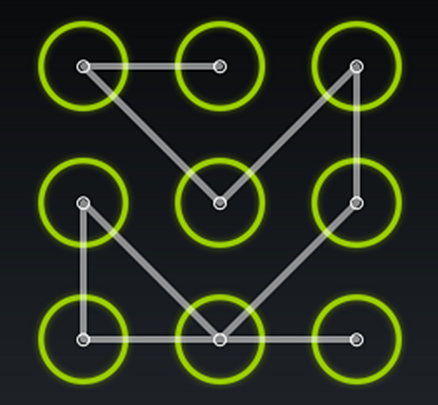
\includegraphics[width=0.2\textwidth]{trace.png} % <- formatos PNG, JPG e PDF
	\small
	\caption[Uso de senha por reconhecimento de padrão]{Uso de senha por reconhecimento de padrão nos \textit{smartphones} Android}
	\label{fig:trace}
\end{figure}

As técnicas (a) e (b) podem ser passíveis de fraude, tendo em vista que alguém possuindo tais informações/objetos pode facilmente conseguir acesso ao sistema como se fosse o verdadeiro usuário. Além disso, esses fatores necessitam da interação direta do usuário, isto é, o usuário deve informar estes dados para realizar a autenticação, geralmente via dispositivos de entrada comuns, como microfone, tela ou teclado.

\subsection{O uso de senhas}
Mesmo a autênticação através do uso de senhas ser o alvo de várias formas de ataque, ela é uma das mais empregadas como meio de assegurar a privacidade de sistemas.
\begin{citacao}
Algumas das formas como a sua senha pode ser descoberta são:
\begin{enumerate}
\item ao ser usada em computadores infectados. Muitos códigos maliciosos, ao infectar um computador, armazenam as teclas digitadas (inclusive senhas), espionam o teclado pela webcam (caso você possua uma e ela esteja apontada para o teclado) e gravam a posição da tela onde o mouse foi clicado;
\item ao ser usada em sites falsos. Ao digitar a sua senha em um site falso, achando que está no site verdadeiro, um atacante pode armazená-la e, posteriormente, usá-la para acessar o site verdadeiro e realizar operações em seu nome;
\item ao ser capturada enquanto trafega na rede, sem estar criptografada;
\item com o uso de técnicas de engenharia social, como forma a persuadi-lo a entregá-la voluntariamente;
\item pela observação da movimentação dos seus dedos no teclado ou dos cliques do mouse em teclados virtuais.
\cite{Cert2016}
\end{enumerate}
\end{citacao}

Para melhorar a eficiência no uso de senhas muitas organizações adotam políticas de segurança que impõem regras no uso das senhas, além disso, criam mecanismos para que as elas tenham um determinado formato, utilizam algum algorítmo de criptografia, expiração de senhas em um determinado tempo, tudo para tentar aumentar a segurança de seus sistemas.

A \sigla{NBR ISO/IEC 27001}{NBR ISO/IEC 27001 - Tecnologia da informação - Técnicas de segurança - Sistemas de gestão de segurança da informação - Requisitos} apresenta aos gestores de segurança da informação sugestões de controles que podem ser adotados nas organizações.

\begin{table}[!htb]
  	\centering
	\label{tab:ISO17}
	\begin{tabular}{|*3{c|}} \hline
		\multicolumn{3}{|c|}{A.11.2 Gerenciamento de acesso do usuário}\\ \hline
		A.11.2.1 & Registro de usuário & \vtop{\hbox{\strut Controle}\hbox{\strut Deve existir um procedimento formal de registro e}\hbox{\strut cancelamento de usuário para garantir e revogar }\hbox{\strut acessos em todos os sistemas de informação}\hbox{\strut e serviços.}} \\ \hline
		A.11.2.3 & \vtop{\hbox{\strut Gerenciamento de}\hbox{\strut senha do usuário}} & \vtop{\hbox{\strut Controle}\hbox{\strut A concessão de senhas deve ser controlada}\hbox{\strut por meio de um processo de gerenciamento formal.}} \\ \hline
	\end{tabular}
	\caption[Objetivos de controle e controles na ABNT NBR ISO/IEC 27001]{Objetivos de controle e controles apresentados na ABNT NBR ISO/IEC 27001 \cite{nbr27001}}
\end{table}

\subsection{O uso de \normalfont\itshape tokens}
O uso de senhas pode não ser seguro o suficiente para garantir a autenticidade e confidencialidade do usuário em alguns tipos de sistemas, como por exemplo o acesso a contas bancárias ou o acesso ao \sigla{SGDB}{Sistema de gerenciamento de banco de dados} de uma aplicação crítica. Nesses sistemas é comum o uso de \textit{tokens}.

\textit{Tokens} são pequenos dispositivos, do tamanho de um chaveiro, cujo nome técnico é \textit{Token} \sigla{OTP}{One Time Password}. Eles geram uma sequência numérica que será utilizada como uma senha mas por um pequeno espaço de tempo, por volta de 60 segundos, depois desse tempo essa sequência numérica perde a validade.

\begin{citacao}
Uma das formas de ataque em sistemas de computação em redes utilizam \textit{softwares} que escutam as conexões para obter informações de autenticação, tais como o \sigla{ID}{Identificação} e senha de usuários. Uma vez que esta informação é capturada, pode ser utilizado mais tarde para obter acesso ao sistema. Sistemas de senha de uso único são projetados para combater este tipo de ataque, chamado de "ataque de repetição".\cite{rfc2289}
\end{citacao}

\begin{figure}[!htb]
	\centering
	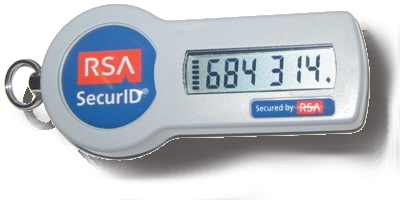
\includegraphics[width=0.22\textwidth]{token.png}
	\small
	\caption[Dispositivo gerador de \textit{tokens}]{Dispositivo gerador de \textit{tokens}}
	\label{fig:token}
\end{figure}

Além dos dispositivos geradores de \textit{tokens} existem também aplicativos que executam a mesma função como é o caso do \textit{Google Authenticator}. Nele são registrados os sistemas ao qual o usuário tem acesso, e quando o usuário precisar acessar algum sistema, ele utiliza a sequência numérica gerada pelo aplicativo.

\begin{figure}[!htb]
	\centering
	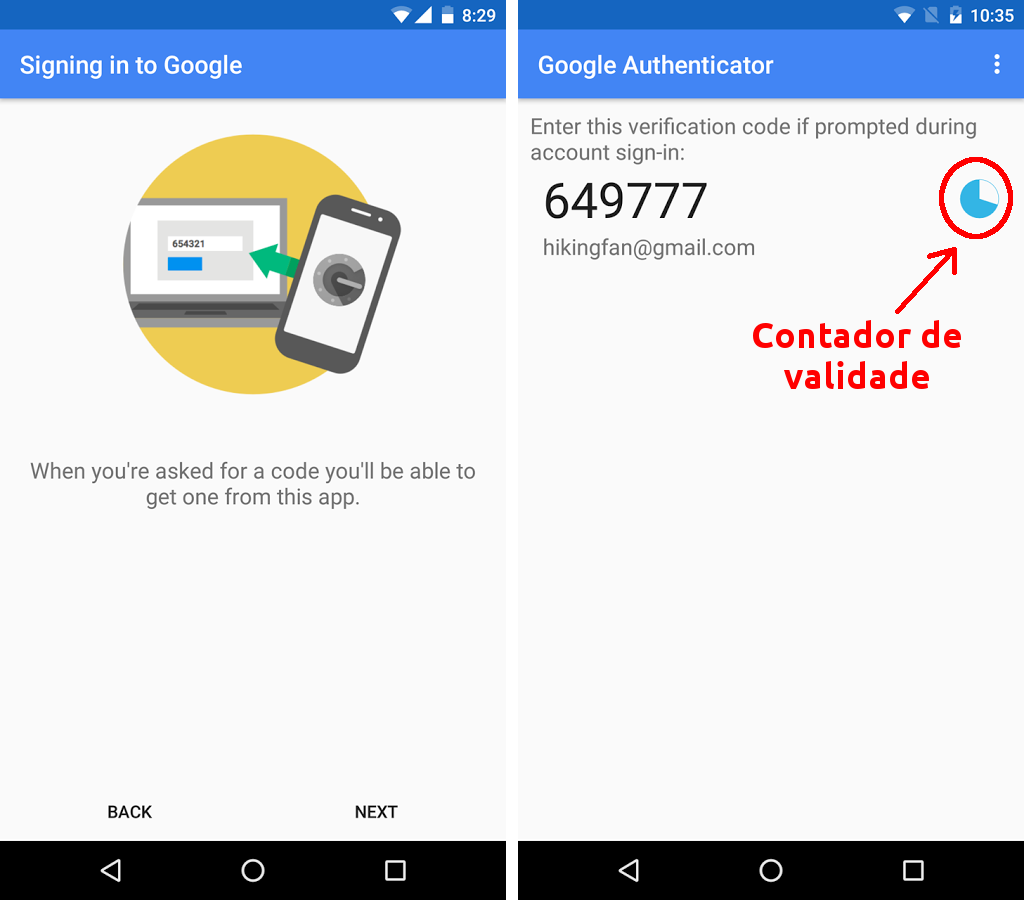
\includegraphics[width=0.46\textwidth]{authenticator.png}
	\small
	\caption[Aplicação geradora de \textit{tokens}]{Aplicação geradora de \textit{tokens}}
	\label{fig:token}
\end{figure}

\subsection{O uso de biometria}
A autenticação por biometria faz o uso de características fisiológicas de cada usuário como por exemplo impressões digitais, reconhecimentos facial, de íris e de voz.
O reconhecimento de algumas dessas características pode negar acesso a um usuário legítimo devido a algumas questões, como por exemplo o uso de barba ou maquiagem que alteram o padrão da face ou um resfriado que pode alterar o padrão da voz.

\begin{citacao}
Como em todos os problemas de reconhecimento de padrões, a questão-chave é a variabilidade: os objetos podem ser classificados de forma confiável apenas se a variabilidade entre diferentes instâncias de uma determinada classe é menor do que a variabilidade entre as diferentes classes. Por exemplo, no reconhecimento de face, as dificuldades surgem a partir do fato de que a face é um órgão social, mutável exibindo uma variedade de expressões. \cite{Daugman2004}
\end{citacao}

Algumas características fisiológicas não têm essa natureza mutável, como é o caso das impressões digitais e os padrões de cores da íris.

\begin{citacao}
Com a utilização da íris como forma de identificação e autenticação de um indivíduo é possível obter um alto grau de segurança e confiabilidade, visto que a íris, além de ser uma característica inerente e única a cada ser humano, permanece inalterada durante toda sua vida, a não ser devido à ocorrência de algum evento externo que possa vir a danificá-la. Isto é, características biométricas são vantajosas sob o ponto de vista de que não precisam ser lembradas, como acontece com as senhas, e nem carregadas, como acontece com os cartões e tokens. \cite{priscila2007}
\end{citacao}

\subsection{Combinação de técnicas de autenticação}
O uso de autenticação por biometria ainda não oferece o custo benefício necessário para ser aplicado em grande escala, pois existe a necessidade de algum tipo de \textit{hardware} especial adicional para que seja possível realizar o reconhecimento.

\begin{figure}[!htb]
	\centering
	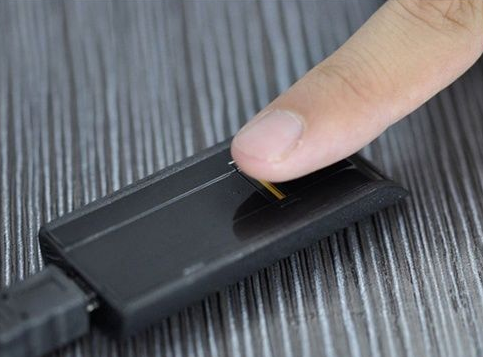
\includegraphics[width=0.3\textwidth]{finger.png}
	\small
	\caption[Leitor biométrico de impressão digital]{Leitor biométrico de impressão digital}
	\label{fig:finger}
\end{figure}

A Figura \ref{fig:finger} apresenta um modelo de um leitor biométrico que pode ser encontrado em lojas virtuas com preços que variam em torno de \sigla{USD}{United States Dollar}20.00. Numa pesquisa por \textit{"iris recognition"}, no Ebay\footnote{http://www.ebay.com}, retornou aparelhos com valores por volta dos USD 1000.00

Como esses aparelhos requerem investimentos, e na grande maioria dos casos os acessos aos sistemas acontecem de diversos pontos, o uso desses aparelhos se torna inviável.
Dessa forma, alguns sistemas utilizam a combinação das técnicas do uso de senha e de \textit{tokens} para aumentar a segurança dos seus sistemas.